\subsection{Ultrafast jet classification at the HL-LHC}
{{\footnotesize
\noindent Demonstrates three ML models (MLP, Deep Sets, Interaction Networks) optimized for FPGA deployment with O(100 ns) inference using quantized models and hls4ml, targeting real-time jet tagging in the L1 trigger environment at the high-luminosity LHC. Data is available on Zenodo DOI:10.5281/zenodo.3602260. 


\begin{description}[labelwidth=4cm, labelsep=1em, leftmargin=4cm, itemsep=0.1em, parsep=0em]
  \item[date:] 2024-07-08
  \item[version:] v1.0
  \item[last\_updated:] 2024-07
  \item[expired:] unknown
  \item[valid:] yes
  \item[valid\_date:] 2024-07-08
  \item[url:] \href{https://arxiv.org/pdf/2402.01876}{https://arxiv.org/pdf/2402.01876}
  \item[doi:] 10.48550/arXiv.2402.01876
  \item[domain:] Particle Physics
  \item[focus:] FPGA-optimized real-time jet origin classification at the HL-LHC
  \item[keywords:]
    - jet classification
    - FPGA
    - quantization-aware training
    - Deep Sets
    - Interaction Networks
  \item[licensing:] CC-BY
  \item[task\_types:]
    - Classification
  \item[ai\_capability\_measured:]
    - Real-time inference under FPGA constraints
  \item[metrics:]
    - Accuracy
    - Latency
    - Resource utilization
  \item[models:]
    - MLP
    - Deep Sets
    - Interaction Network
  \item[ml\_motif:]
    - Real-time
  \item[type:] Model
  \item[ml\_task:]
    - Supervised Learning
  \item[solutions:] Solution details are described in the referenced paper or repository.
  \item[notes:] Uses quantization-aware training; hardware synthesis evaluated via hls4ml

  \item[contact.name:] Patrick Odagiu
  \item[contact.email:] podagiu@ethz.ch
  \item[datasets.links.name:] Zenodo dataset
  \item[datasets.links.url:] \href{https://zenodo.org/records/3602260}{https://zenodo.org/records/3602260}
  \item[results.links.name:] ChatGPT LLM
  \item[results.links.url:] \href{https://docs.google.com/document/d/1gDf1CIYtfmfZ9urv1jCRZMYz\_3WwEETkugUC65OZBdw}{https://docs.google.com/document/d/1gDf1CIYtfmfZ9urv1jCRZMYz\_3WwEETkugUC65OZBdw}
  \item[fair.reproducible:] True
  \item[fair.benchmark\_ready:] False
  \item[id:] ultrafast\_jet\_classification\_at\_the\_hl-lhc
  \item[Citations:] \cite{odagiu2024ultrafastjetclassificationfpgas}
\end{description}

{\bf Ratings:} ~ \\

\begin{tabular}{p{0.15\textwidth} p{0.07\textwidth} p{0.7\textwidth}}
\hline
Rating & Value & Reason \\
\hline
dataset & 4 & FAIR metadata limited; no clear mention of dataset format or splits
 \\
documentation & 3 & No linked GitHub repo or setup instructions; paper provides partial guidance only
 \\
metrics & 3 & Metrics exist (accuracy, latency, utilization), but formal definitions and evaluation guidance are limited
 \\
reference\_solution & 2 & Reference implementations not fully reproducible; no evaluation pipeline or training setup provided
 \\
software & 3 & Not containerized; Setup and automation incomplete
 \\
specification & 4 & Hardware constraints are referenced but not fully detailed or standardized
 \\
\hline
\end{tabular}

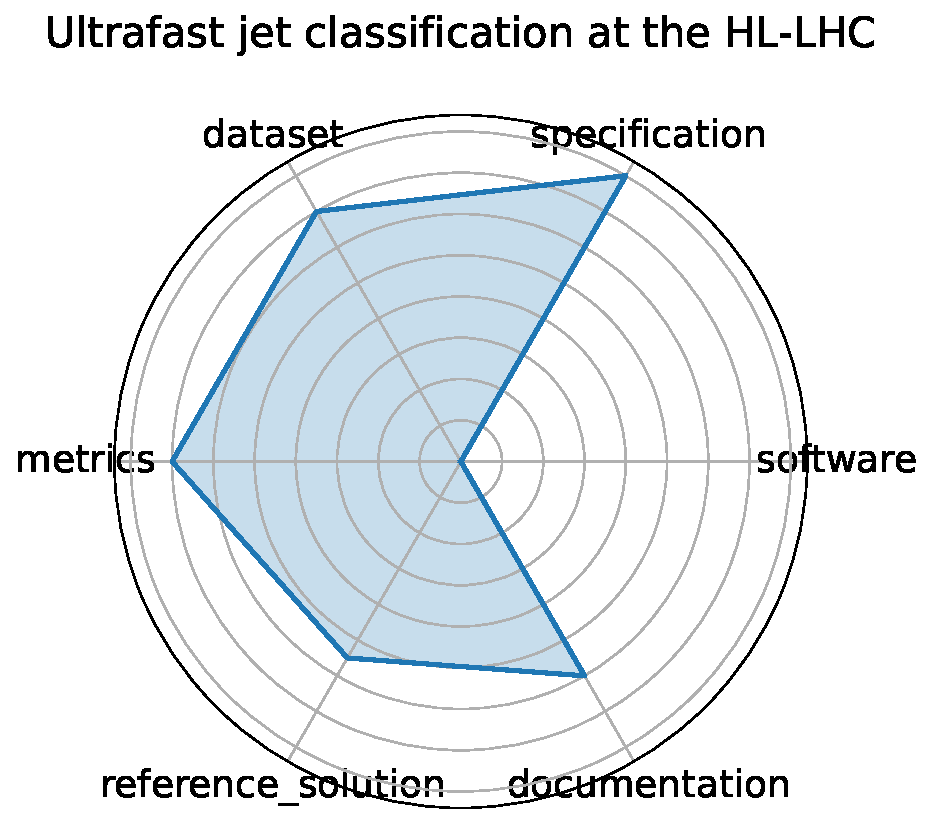
\includegraphics[width=0.2\textwidth]{ultrafast_jet_classification_at_the_hl-lhc_radar.pdf}
}}
\clearpage